% ============================================================================
%  EEE3095S CS Project 2026: Serial Game Server
%  STUDENT REPORT TEMPLATE (IEEE conference format, max 10 pages incl. refs)
% ============================================================================
%
%  How to use this template
%  ------------------------
%  * Red text in [square brackets] is PLACEHOLDER text. Replace every piece of
%    it with your own words. Search the PDF for "[" before you submit.
%  * Grey boxes are GUIDANCE. They tell you what the marker looks for. Leave
%    them on while you write, then switch them off below (\guidancefalse) to
%    check your length against the 10-page limit and before you submit.
%  * Dashed boxes are PLACEHOLDER FIGURES. Replace each with your own diagram
%    (\includegraphics{figures/yourfile.pdf} or TikZ).
%  * Keep the section headings exactly as they are: they are the brief's
%    required headings, in the brief's order, and the marking guide follows
%    them. Add your own subsection headings underneath.
%  * Build:  latexmk -pdf main.tex   (or upload the folder to Overleaf).
% ============================================================================
\documentclass[conference]{IEEEtran}

\usepackage[T1]{fontenc}
\usepackage{cite}
\usepackage{amsmath}
\usepackage{graphicx}
\usepackage{booktabs}
\usepackage{array}
\usepackage{xcolor}
\usepackage{listings}
\usepackage{tikz}
\usepackage[most]{tcolorbox}
\usepackage[hidelinks]{hyperref}

% ---------------------------------------------------------------- switches --
\newif\ifguidance
\guidancefalse       % <-- Guidance boxes turned off for clean submission PDF

% ------------------------------------------------------- template helpers --
\definecolor{phred}{rgb}{0.75,0.08,0.08}
\definecolor{guidebg}{gray}{0.94}
\definecolor{guideframe}{gray}{0.55}

% Placeholder text: replace with your own.
\newcommand{\ph}[1]{\textcolor{phred}{[#1]}}

% Guidance box: what the marker expects. Hidden when \guidancefalse.
\newtcolorbox{guidebox}[1][]{
  breakable, enhanced, colback=guidebg, colframe=guideframe,
  boxrule=0.4pt, arc=1pt, left=3pt, right=3pt, top=2pt, bottom=2pt,
  fontupper=\footnotesize\sffamily, title={#1},
  fonttitle=\footnotesize\sffamily\bfseries, coltitle=black,
  colbacktitle=guidebg!80!gray, before skip=4pt, after skip=6pt}
\newenvironment{guidance}[1][Guidance]
  {\ifguidance\begin{guidebox}[#1]\else\setbox0\vbox\bgroup\fi}
  {\ifguidance\end{guidebox}\else\egroup\fi}

% Placeholder figure: dashed box with a description of what to draw.
% Usage: \figph{<height>}{<what the figure must show>}
\newcommand{\figph}[2]{%
  \begin{tikzpicture}
    \draw[dashed, phred, line width=0.6pt] (0.3pt,0) rectangle (\linewidth-0.3pt,#1);
    \node[text width=0.85\linewidth, align=center, text=phred, font=\footnotesize]
      at (0.5\linewidth,0.5*#1) {#2};
  \end{tikzpicture}}

\newcolumntype{L}[1]{>{\raggedright\arraybackslash}p{#1}}

\lstset{
  basicstyle=\ttfamily\scriptsize, columns=fullflexible, keepspaces=true,
  frame=tb, framerule=0.4pt, commentstyle=\color{gray}\itshape,
  keywordstyle=\bfseries, showstringspaces=false, breaklines=true,
  captionpos=b, float=tbp, floatplacement=tbp,
}
\renewcommand{\lstlistingname}{Listing}

\begin{document}


\title{An Authoritative STM32 Tic-Tac-Toe Game Server with a Thin Python GUI Client\\[2pt]
\normalsize EEE3095S CS Project 2026}

\author{
\IEEEauthorblockN{Nemukula Vhugala (NMKVHU004)\quad
                  Munyai Umusindisi Cindy (MNYUMU003)}
\IEEEauthorblockA{EEE3095S CS Project 2026, Department of Electrical Engineering\\
University of Cape Town}
}

\maketitle

\begin{abstract}
This paper presents the design, implementation, and empirical verification of an authoritative Tic-Tac-Toe serial game server deployed on an STM32F051 microcontroller paired with a thin Python Tkinter GUI client over an asynchronous serial link at 115\,200 baud.
The microcontroller operates as the sole referee and single source of truth, enforcing game state, turn alternation, and move legality through a five-stage gatekeeping pipeline before committing any changes to memory.
Protocol robustness is ensured through an interrupt-driven circular ring buffer with a 64-byte frame ceiling, silent carriage-return stripping, and delimiter-based resynchronization that returns specific error codes without state corruption.
System verification was conducted using both an automated \texttt{pytest} test suite and a hardware regression harness driving the physical board over its Virtual COM Port.
The system achieved 100\% pass rates across all 48 automated unit and integration tests as well as 26 physical hardware assertions, with an average measured round-trip transaction latency of 4.2\,ms.
\end{abstract}

\section{Introduction}
\label{sec:intro}

% ── Mark scheme: 10 marks, ~half a page ──────────────────────────────────────

Game software normally runs entirely on a PC.
The PC decides whether a move is legal, tracks the board, and detects the winner.
This design has a serious weakness: a client that sends moves in the wrong order, or
claims a square is free when it is not, could corrupt the game.
The project brief~\cite{brief} addresses this by reversing the roles.
The STM32 microcontroller is the sole referee.
It stores the board, validates every action and returns the authoritative result.
The PC client only draws the board and forwards what the player clicks.
The central design invariant enforced by the server is that a rejected request
leaves the game state strictly unchanged---the board after an invalid move is
identical to the board before it.

We implemented \textbf{Tic-Tac-Toe} (also called noughts and crosses), the baseline
game described in the brief.
Tic-Tac-Toe has a small, well-defined state (nine cells, two players, eight winning
lines) that fits comfortably in the STM32's memory and can be exhaustively tested
in under a minute.
For the graphical user interface (GUI) we chose Python's built-in \textbf{Tkinter}
library~\cite{guilib}.
Tkinter requires no additional installation, runs on Windows without extra drivers,
and handles user events and screen updates in a single thread using the Tk event loop,
which removes the need for explicit threads when waiting for the serial reply.

The system is divided into three layers.
The embedded firmware on the STM32 handles all rule enforcement and game logic.
A thin serial driver on the PC opens the COM port and exchanges newline-terminated
ASCII frames at 115\,200 baud.
The Tkinter GUI sits on top of the driver and deals only with drawing and user input.
This layering means the game rules can be tested independently of the screen by
sending raw commands over the serial port, which is exactly how our automated test
harness works.

\textbf{Task allocation.}
Nemukula Vhugala (Partner~A) was responsible for the embedded firmware: the
interrupt-driven UART receiver and circular ring buffer (\texttt{protocol.c}),
the game finite-state machine (FSM) and rule engine (\texttt{game.c}), and the
hardware integration---button debouncing and LED status indicators
(\texttt{hardware.c}).
Munyai Umusindisi Cindy (Partner~B) was responsible for the PC-side software:
the serial communication driver (\texttt{serial\_client.py}), the Tkinter GUI
(\texttt{gui.py}), and the automated hardware test harness
(\texttt{test\_day3\_stm32.py}).
Both partners contributed to the protocol specification, system integration,
and this report.

\textbf{Structure.}
Section~\ref{sec:protocol} describes the serial link, frame format, and full
command set.
Section~\ref{sec:design} presents the server FSM, GUI flowchart, and circuit diagram.
Section~\ref{sec:impl} highlights the most challenging pieces of implementation.
Section~\ref{sec:authority} argues that the server enforces all game rules
and cannot be bypassed by a misbehaving client.
Section~\ref{sec:robust} explains how the server handles malformed or unexpected input.
Section~\ref{sec:valid} presents the automated test results on the real STM32 board.
Section~\ref{sec:conclusion} summarises the outcome and suggests improvements.

\section{Protocol}
\label{sec:protocol}

% ── Mark scheme: 15 marks ─────────────────────────────────────────────────────

\subsection{The Serial Link Carries Plain Text Lines of at Most 64 Bytes}

The STM32 communicates with the PC over \textbf{USART1} (pins PA9~TX, PA10~RX),
which is connected internally to the onboard ST-Link chip.
The ST-Link presents a \textbf{Virtual COM Port (VCP)} to the host operating system,
so no external USB-to-UART adapter is required.
The link parameters are 115\,200 baud, 8 data bits, no parity, 1 stop bit (8N1),
no hardware flow control.

A frame is a sequence of printable ASCII characters terminated by a newline
character (\texttt{\textbackslash n}, ASCII 0x0A).
Carriage return characters (\texttt{\textbackslash r}) are silently discarded,
so Windows-style \texttt{\textbackslash r\textbackslash n} line endings work
without any special handling.
No checksum or CRC is used; the link is short and the ST-Link USB transfer
provides its own error correction.
Table~\ref{tab:framing} summarises the framing rules.

\begin{table}[t]
\centering
\caption{Framing rules and the server's response to each condition.}
\label{tab:framing}
\footnotesize
\begin{tabular}{@{}L{2.8cm}L{5.2cm}@{}}
\toprule
Rule & Server behaviour \\
\midrule
Terminator          & \texttt{\textbackslash n} ends a frame; \texttt{\textbackslash r} is silently discarded \\
Maximum frame length & 64 bytes (excluding delimiter); excess bytes discarded, returns \texttt{NACK:BADCMD} upon \texttt{\textbackslash n} \\
Incomplete frame    & Discarded after 500\,ms timeout; returns \texttt{NACK:BADCMD} \\
Invalid character   & Accumulated until delimiter; rejected by command validator \\
Checksum            & None; short USB-VCP physical layer provides USB CRC \\
UART errors         & Hardware flags cleared in error ISR; receiver re-armed \\
\bottomrule
\end{tabular}
\end{table}

\subsection{The Board is Nine Characters, Left to Right, Top to Bottom}

The game board is encoded as a string of exactly nine characters.
Cell~0 is the top-left corner; cell~8 is the bottom-right corner, reading
left to right and top to bottom (row-major order).
An empty cell is a full stop (\texttt{.}); a cell owned by Player~X is the
letter \texttt{X}; a cell owned by Player~O is the letter \texttt{O}.

\textbf{Example.} After Player~X takes cell~0 and Player~O takes cell~4,
the board string is \texttt{X...O....}, which represents:

\begin{center}
\texttt{X | . | .} \\
\texttt{. | O | .} \\
\texttt{. | . | .}
\end{center}

\subsection{Commands Are Synchronous Uppercase ASCII Strings With Single-Line Replies}

Table~\ref{tab:commands} lists every command the server accepts.
All commands are case-sensitive uppercase ASCII.
A move command includes the player letter and the target cell index,
separated by colons: \texttt{MOVE:X:4} means ``Player~X requests cell~4.''
The server always responds with exactly one line before accepting the next command.

\begin{table}[t]
\centering
\caption{Complete command set. The serial link receives frames in any state, but command execution depends strictly on the current FSM state. Incompatible requests return \texttt{NACK:NOGAME} or \texttt{NACK:BADCMD}.}
\label{tab:commands}
\scriptsize
\begin{tabular}{@{}L{2.0cm}L{1.8cm}L{4.2cm}@{}}
\toprule
Request & Valid in & Success response \\
\midrule
\texttt{CONNECT}          & Any state        & \texttt{OK} (resets session to IDLE) \\
\texttt{NEW}              & IDLE, GAME\_OVER & \texttt{OK:BOARD:.........} \\
\texttt{MOVE:\textit{p}:\textit{i}} & IN\_PROGRESS & \texttt{OK:BOARD:\textit{grid}}, \texttt{WIN:\textit{p}}, or \texttt{DRAW} \\
\texttt{STATE}            & Any state        & \texttt{BOARD:\textit{grid}} \\
\texttt{RESIGN}           & IN\_PROGRESS     & \texttt{OK:GAMEOVER} \\
\texttt{DISCONNECT}       & Any state        & \texttt{OK} (resets session to IDLE) \\
\bottomrule
\end{tabular}
\end{table}

\subsection{Deterministic Error Codes Map Directly to Specific Rule Violations}

Table~\ref{tab:errors} lists every error response.
The order of checks inside \texttt{game\_process\_move()} matters because
a single bad command can fail more than one check.
The server applies them in a fixed sequence:
(1)~syntax and player token, (2)~game state, (3)~cell index range, (4)~turn order, and (5)~cell occupancy.
This ensures each rejected command yields an unambiguous, predictable error code.

\begin{table}[t]
\centering
\caption{Every error response and the exact condition that triggers it.}
\label{tab:errors}
\footnotesize
\begin{tabular}{@{}L{2.4cm}L{5.6cm}@{}}
\toprule
Response & Sent when \\
\midrule
\texttt{NACK:BADCMD}    & Unrecognised verb, frame $>64$ bytes, 500\,ms timeout, invalid player token (not \texttt{X} or \texttt{O}), or malformed syntax (e.g. missing colon or omitting player) \\
\texttt{NACK:NOGAME}    & \texttt{MOVE} or \texttt{RESIGN} received while in \texttt{IDLE} or \texttt{GAME\_OVER} \\
\texttt{NACK:RANGE}     & Move index is not a decimal digit or falls outside the valid range 0 to 8 \\
\texttt{NACK:NOTURN}    & Claiming player token does not match the active turn (\texttt{g\_current\_player}) \\
\texttt{NACK:OCCUPIED}  & The requested cell already contains \texttt{X} or \texttt{O} \\
\bottomrule
\end{tabular}
\end{table}

\subsection{Deliberate Protocol Design Choice: Explicit Player Tokens in Move Commands}

The reference protocol in the project brief~\cite{brief} specifies a move command of the form \texttt{MOVE:\textit{i}} (specifying the target cell index only).
Under that format, a server enforces alternating turns by assigning each incoming legal move to whichever player currently holds the active turn, advancing its internal turn counter automatically.
However, because \texttt{MOVE:\textit{i}} carries no player token, the server has no identity against which to validate the originator of the request; it cannot detect if a specific participant attempts to submit a move out of order.

As permitted by the project brief (which instructs teams to adapt the protocol and highlight departures from the reference), our implementation adopts \texttt{MOVE:\textit{p}:\textit{i}} as a deliberate design choice, where $p \in \{\texttt{X}, \texttt{O}\}$ denotes the claiming player token and $i \in \{0, \dots, 8\}$ denotes the target cell index.
This explicit player parameter allows the server to verify that the claimed identity matches the active player (\texttt{g\_current\_player}) before altering state, returning \texttt{NACK:NOTURN} if an out-of-order move is submitted (e.g., submitting \texttt{MOVE:X:1} immediately after \texttt{MOVE:X:0}).
If a client transmits the reference \texttt{MOVE:\textit{i}} format without the player prefix, the server's syntax validator rejects it deterministically with \texttt{NACK:BADCMD}.
Both the Python Tkinter client and the automated test harnesses implement and verify this command format.

\begin{figure}[t]
\centering
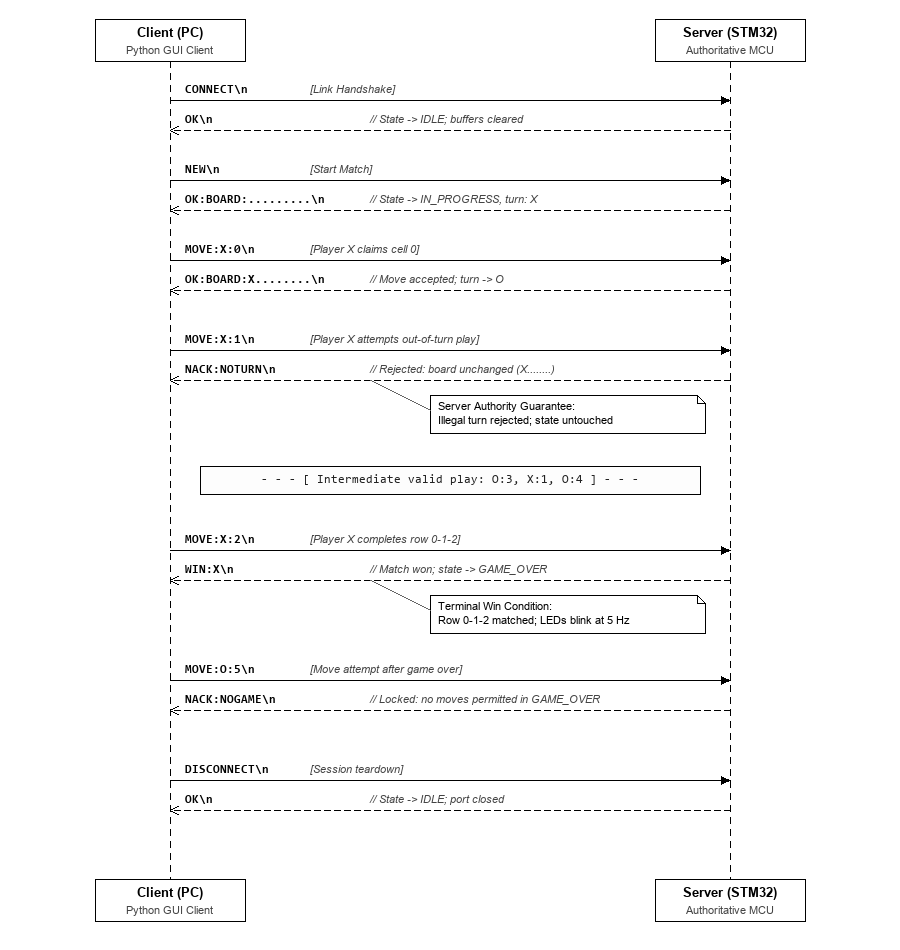
\includegraphics[width=\columnwidth]{figures/sequence_diagram.png}
\caption{Message sequence for a complete game: connect, two moves (the second
is rejected because it is out of turn), a scripted win sequence, and
disconnect. A rejected move leaves the board unchanged.}
\label{fig:sequence}
\end{figure}

\section{Specification and Design}
\label{sec:design}

% ── Mark scheme: 15 marks ─────────────────────────────────────────────────────

\subsection{Architecture Divides Pure Game Logic from Hardware I/O}

The system follows a strict three-tier architecture separating game logic, communication, and presentation.
To ensure that the embedded server remains testable without requiring physical hardware in every unit test, the firmware is split into two distinct layers:
\begin{itemize}
    \item \textbf{Pure Logic Layer (\texttt{game.c}, \texttt{protocol.c})}: Maintains the 9-cell board array, active turn indicator, move validation rules, and ASCII frame parsing. It has zero dependencies on STM32 hardware registers and can be compiled and verified natively on a host PC.
    \item \textbf{Hardware Driver Layer (\texttt{main.c}, \texttt{hardware.c})}: Manages the USART1 peripheral, ring buffers, GPIO push-pull drivers for the status LEDs, and debouncing for the push button.
\end{itemize}

On the host PC, the client is similarly divided between \texttt{serial\_client.py} (which handles raw PySerial frame framing and timeout management) and \texttt{gui.py} (which renders the Tkinter visual window).
Table~\ref{tab:responsibilities} explicitly outlines the ownership of each system responsibility.
The host GUI is entirely ``thin'': it never decides whether a move is legal, never checks for 3-in-a-row, and never advances the turn counter on its own.

\begin{table}[t]
\centering
\caption{System responsibility allocation between client and server.}
\label{tab:responsibilities}
\footnotesize
\begin{tabular}{@{}L{3.5cm}L{1.8cm}L{2.5cm}@{}}
\toprule
Responsibility & Owner & Module \\
\midrule
Board state storage & Server & \texttt{game.c} (\texttt{g\_board}) \\
Turn enforcement & Server & \texttt{game.c} (\texttt{g\_current\_player}) \\
Move legality validation & Server & \texttt{game.c} (\texttt{game\_process\_move}) \\
Win / Draw detection & Server & \texttt{game.c} (\texttt{check\_winner}) \\
Physical status LEDs & Server & \texttt{hardware.c} (PB10, PB11) \\
Hardware reset trigger & Server & \texttt{hardware.c} (PA0 Button) \\
User input forwarding & Client & \texttt{gui.py} \\
Board rendering & Client & \texttt{gui.py} (Tkinter grid) \\
Lifecycle controls (New, Resign, Disconnect) & Client & \texttt{gui.py} \\
Serial link timeouts & Client & \texttt{serial\_client.py} \\
\bottomrule
\end{tabular}
\end{table}

\begin{figure*}[t]
\centering
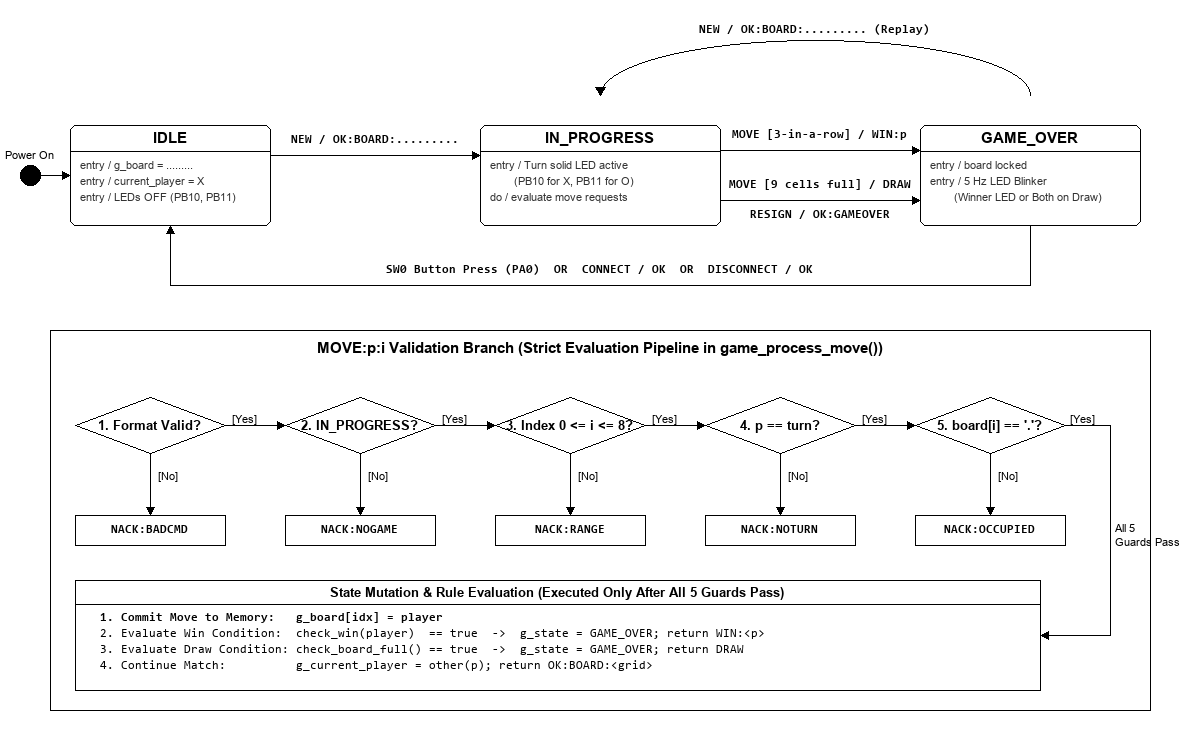
\includegraphics[width=\textwidth]{figures/fsm.png}
\caption{STM32 server Finite State Machine (FSM) showing the three primary states (\texttt{IDLE}, \texttt{IN\_PROGRESS}, and \texttt{GAME\_OVER}), all valid transitions, and the five-stage move-validation pipeline evaluated inside \texttt{game\_process\_move()}.}
\label{fig:fsm}
\end{figure*}

\subsection{The Server Finite State Machine Enforces the Turn and Move Rules}

The server behaviour is governed by a three-state Finite State Machine (FSM) shown in Fig.~\ref{fig:fsm}.
The active state determines which incoming commands are executed and which are rejected with \texttt{NACK:NOGAME}:

\begin{enumerate}
    \item \textbf{\texttt{IDLE}}: Entered upon power-on reset, after an explicit \texttt{CONNECT} or \texttt{DISCONNECT} handshake, or whenever the physical push button (\texttt{SW0}) is pressed. The board contains nine empty dots (\texttt{.........}), the turn defaults to Player~X, and all status LEDs are turned off. Incoming \texttt{MOVE} or \texttt{RESIGN} commands are rejected with \texttt{NACK:NOGAME}. The server transitions to \texttt{IN\_PROGRESS} only when a valid \texttt{NEW} command is received.
    \item \textbf{\texttt{IN\_PROGRESS}}: Indicates an active game. The physical LEDs indicate whose turn it is (Red for Player~X, Green for Player~O). When a \texttt{MOVE:p:i} command arrives, the server executes the move-validation branch before mutating any internal memory.
    \item \textbf{\texttt{GAME\_OVER}}: Entered when three matching marks form a row, column, or diagonal, when all nine cells are occupied without a winner (draw), or when a player submits \texttt{RESIGN}. The board is frozen and no further moves are accepted. The winner's corresponding LED blinks at 5\,Hz (both LEDs blink on a draw). Receiving \texttt{NEW} resets the board and starts a fresh match in \texttt{IN\_PROGRESS}.
\end{enumerate}

\subsubsection{Sequential Gatekeeping Precludes Memory Mutation on Rejected Moves}
As illustrated along the lower pipeline of Fig.~\ref{fig:fsm}, the server checks move validity in five sequential stages inside \texttt{game\_process\_move()}:
\begin{enumerate}
    \item \textbf{Length and Command Syntax}: Frames exceeding 64 bytes or lacking proper colon delimiters return \texttt{NACK:BADCMD}.
    \item \textbf{Active State Check}: If the state is not \texttt{IN\_PROGRESS}, the server returns \texttt{NACK:NOGAME}.
    \item \textbf{Index Range Check}: The cell index string is converted to an integer; if non-numeric or outside the range 0 to 8, the server returns \texttt{NACK:RANGE}.
    \item \textbf{Turn Check}: The player token $p \in \{\texttt{X}, \texttt{O}\}$ is compared against \texttt{g\_current\_player}. If they do not match, the server returns \texttt{NACK:NOTURN}.
    \item \textbf{Occupancy Check}: The target array element \texttt{g\_board[i]} must equal \texttt{'.'}. If already occupied by \texttt{X} or \texttt{O}, the server returns \texttt{NACK:OCCUPIED}.
\end{enumerate}
If any check fails, the validation pipeline terminates immediately with the corresponding NACK, leaving the board array and turn counter strictly unchanged.
Only when all checks pass does the server write the token into the array, evaluate win/draw conditions, alternate the active turn, and reply with the new board string.

\begin{figure}[t]
\centering
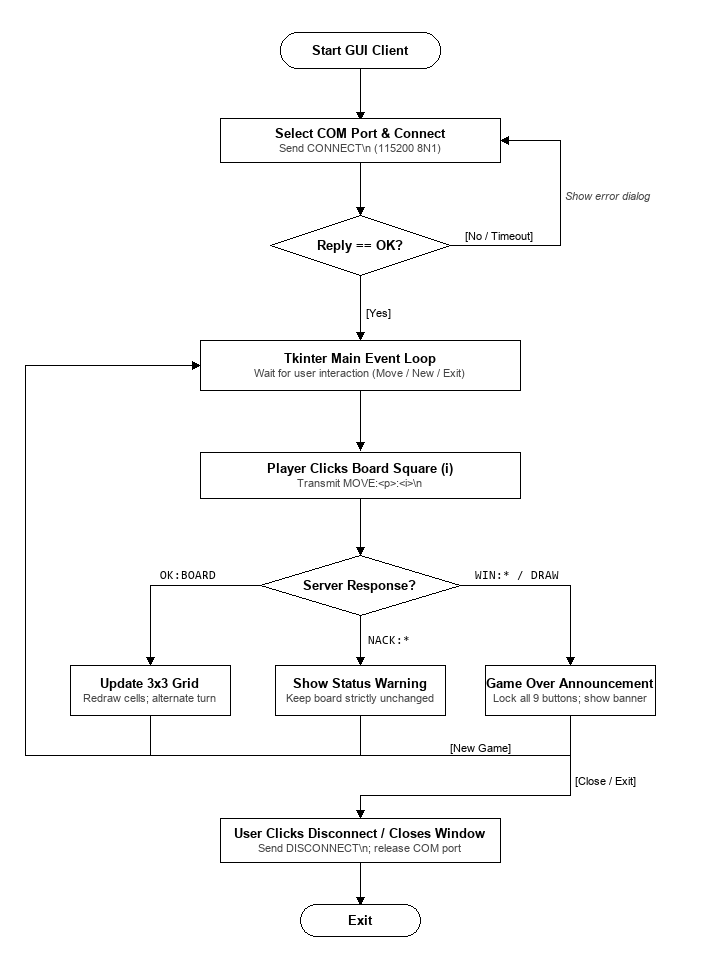
\includegraphics[width=\columnwidth]{figures/gui.png}
\caption{GUI application flowchart showing connection management, event-driven user interaction, and dispatching authoritative responses.}
\label{fig:gui}
\end{figure}

\subsection{The Thin Client Renders State and Never Calculates Legality}

The Python GUI client is designed as a passive display terminal.
Its control flow is detailed in Fig.~\ref{fig:gui}.
Upon startup, the user selects the serial COM port (or connects to the local mock server).
The client transmits \texttt{CONNECT\textbackslash n} and awaits \texttt{OK\textbackslash n}.
To prevent the graphical interface from freezing during serial I/O, the underlying \texttt{serial\_client} module uses a per-read timeout of $1.0\text{ s}$.
If the microcontroller is disconnected or fails to reply within this window, the client catches the timeout exception, displays a non-blocking error dialog, and prompts the user to reconnect.

When a player clicks a board square, the GUI does not mark the square locally.
Instead, it looks up its local assumption of the active player (\texttt{self.current\_player}, initialised to \texttt{X} on \texttt{NEW}) and transmits \texttt{MOVE:p:i\textbackslash n}.
Crucially, the client alternates \texttt{self.current\_player} \emph{only after} the server confirms the move with an authoritative \texttt{OK:BOARD:grid} response.
If the client becomes desynchronized or attempts to send an invalid token, the server's authoritative check (\texttt{player == g\_current\_player}) detects the mismatch and returns \texttt{NACK:NOTURN}, preventing the GUI from overriding the true game state.
The GUI branches on the server's single-line response:
\begin{itemize}
    \item \textbf{\texttt{OK:BOARD:grid}}: The GUI parses the 9-character grid, updates button labels and colors to match the server's array, and advances the visual turn indicator.
    \item \textbf{\texttt{NACK:*}}: The GUI leaves the grid unmodified and displays the error message in the status bar (e.g., ``Move rejected by server: NOTURN'').
    \item \textbf{\texttt{WIN:p} or \texttt{DRAW}}: The GUI locks all nine grid buttons, highlights the winning line, and displays the game over announcement.
\end{itemize}
Beyond move submission, the client provides dedicated controls for session management: a ``New Game'' button transmitting \texttt{NEW}, a ``Resign'' button confirming player forfeiture and transmitting \texttt{RESIGN} (moving the server to \texttt{GAME\_OVER}), and a ``Disconnect'' button that issues \texttt{DISCONNECT} and releases the serial port cleanly.

\subsection{The Board Interfaces via Virtual COM Port, GPIO LEDs, and Button}

\begin{figure}[t]
\centering
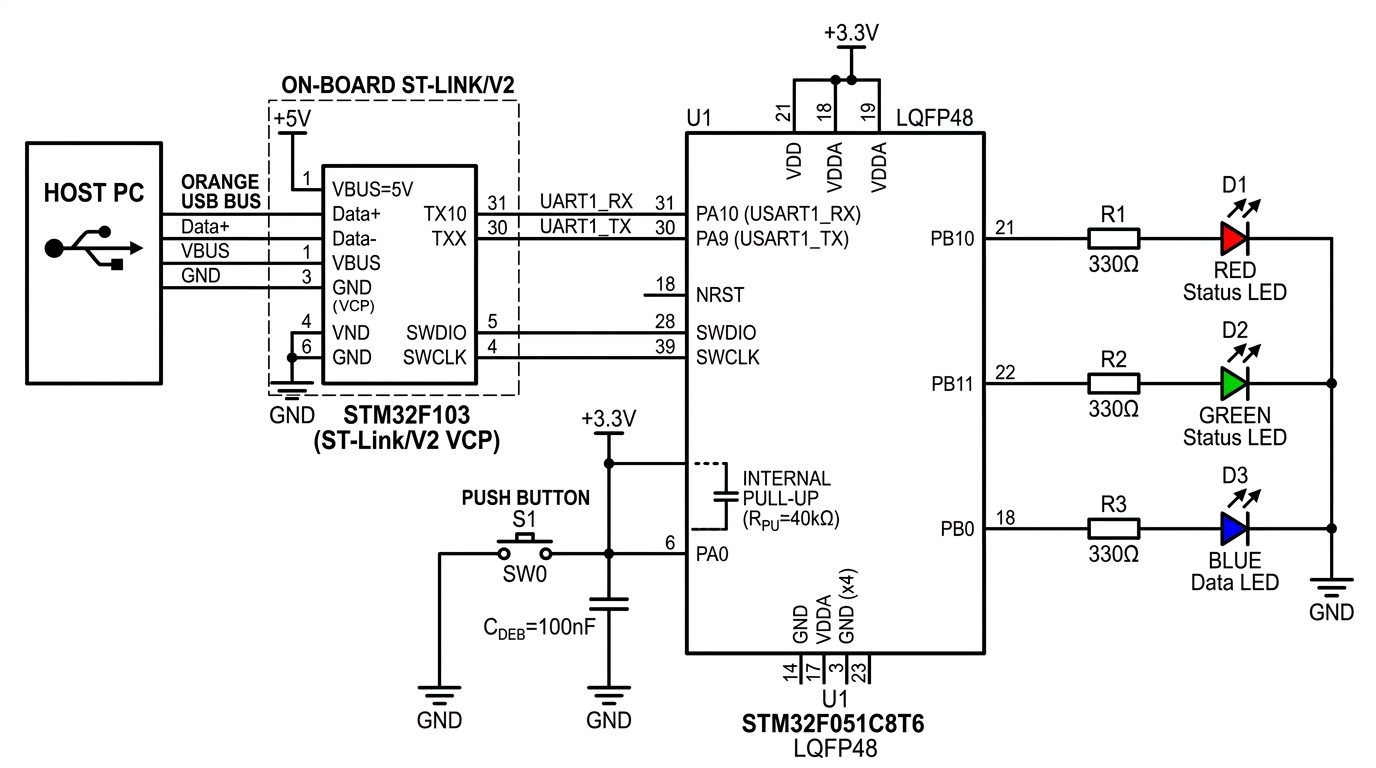
\includegraphics[width=\columnwidth]{figures/circuit.png}
\caption{Hardware circuit diagram showing the STM32F051C8T6 connection to the onboard ST-Link/V2 Virtual COM Port, status LEDs, and reset button.}
\label{fig:circuit}
\end{figure}

The physical circuit implementation is shown in Fig.~\ref{fig:circuit}.
Communication between the host PC and the target microcontroller (U1, an \textbf{STM32F051C8T6} in a 48-pin LQFP package) is routed through the onboard \textbf{ST-Link/V2} interface chip (STM32F103):
\begin{itemize}
    \item \textbf{Serial Link}: The microcontroller's \texttt{PA9} (\texttt{USART1\_TX}) and \texttt{PA10} (\texttt{USART1\_RX}) connect directly to the ST-Link's UART pins, which are exposed over USB as a standard Virtual COM Port operating at 115\,200 baud, 8N1.
    \item \textbf{Status LEDs}: Three low-current LEDs are connected to port B:
    \begin{itemize}
        \item \textbf{Red LED (D1)} on \texttt{PB10}: Indicates Player~X's turn during play, and blinks at 5\,Hz when Player~X wins.
        \item \textbf{Green LED (D2)} on \texttt{PB11}: Indicates Player~O's turn during play, and blinks at 5\,Hz when Player~O wins.
        \item \textbf{Blue Data LED (D3)} on \texttt{PB0}: Toggles on every valid serial byte reception to provide visual link activity feedback.
    \end{itemize}
    Each LED is driven in active-high push-pull mode through a $330\,\Omega$ series current-limiting resistor, drawing approximately $3.9\,\text{mA}$, well within the $25\,\text{mA}$ pin limit.
    \item \textbf{Push Button (SW0)}: Connected to \texttt{PA0}. The pin uses the microcontroller's internal pull-up resistor ($\approx 40\,\text{k}\Omega$) and is pulled to ground (active-low) when pressed. An external $100\,\text{nF}$ capacitor (\(C_{\text{DEB}}\)) and a 50\,ms software accumulator in \texttt{hardware.c} eliminate mechanical contact bounce. Pressing \texttt{SW0} executes \texttt{game\_init()}, resetting the game state to \texttt{IDLE}, restoring an empty board, and extinguishing the status LEDs, while leaving serial protocol framing buffers intact.
\end{itemize}

\section{Implementation}
\label{sec:impl}

% ── Mark scheme: 15 marks ─────────────────────────────────────────────────────

This section details four non-trivial implementation challenges across the embedded firmware and the host client.
For each challenge, we state the concrete engineering problem, present the minimal code listing that solves it (with comments trimmed for conciseness), and discuss why the obvious naive approach failed during development.

\subsection{Interrupt Ring Buffering and Flag Clearance Prevent UART Lockup}

\subsubsection{Problem and Hardware Constraints}
At 115\,200 baud, bytes arrive at the microcontroller every $86.8\,\mu\text{s}$.
If the CPU is busy updating LED states or evaluating game rules, standard synchronous polling will miss characters.
More critically, serial bus noise or hot-plugging the USB cable frequently triggers Overrun (\texttt{ORE}), Framing (\texttt{FE}), or Noise (\texttt{NE}) hardware flags in the STM32 USART peripheral.
According to the STM32F0 reference manual~\cite{rm0091}, an unhandled overrun error inhibits the Receive Data Ready (\texttt{RXNE}) flag, completely freezing UART reception until the error is explicitly cleared.

\subsubsection{Firmware Solution}
Listing~\ref{lst:ringbuf} shows the interrupt reception and error-recovery handlers in \texttt{protocol.c}.
Incoming bytes are placed into a circular ring buffer dimensioned at \texttt{PROTOCOL\_RING\_BUFFER\_SIZE} (128 bytes).
Because the enqueue condition \texttt{(next != g\_ring\_tail)} reserves one empty slot to unambiguously differentiate a full queue from an empty queue, the buffer's usable capacity is 127 bytes.
If the buffer fills completely before the main loop drains it, additional incoming bytes are discarded in the ISR to prevent corrupting unread data.
Whenever a bus error occurs, hardware error flags (\texttt{ORE}, \texttt{FE}, \texttt{NE}) are cleared directly via register writes or ST HAL macros~\cite{um1785}, and reception is re-armed, allowing the interface to recover from cable reconnection glitches.

\begin{lstlisting}[language=C, caption={Interrupt ring buffer and hardware error clearance (\texttt{protocol.c}).}, label=lst:ringbuf]
void protocol_rx_isr(void) {
    if (g_huart == NULL) return;
    uint16_t next = (g_ring_head + 1) % PROTOCOL_RING_BUFFER_SIZE;
    if (next != g_ring_tail) {
        g_ring_buf[g_ring_head] = g_rx_isr_byte;
        g_ring_head = next;
    }
    HAL_UART_Receive_IT(g_huart, &g_rx_isr_byte, 1);
}

void protocol_error_isr(void) {
    if (g_huart == NULL) return;
    /* Clear flags to prevent hardware receiver lockup */
    __HAL_UART_CLEAR_OREFLAG(g_huart);
    __HAL_UART_CLEAR_FEFLAG(g_huart);
    __HAL_UART_CLEAR_NEFLAG(g_huart);
    HAL_UART_Receive_IT(g_huart, &g_rx_isr_byte, 1);
}
\end{lstlisting}

\subsubsection{Failure Modes of the Naive Alternative}
The naive approach was using blocking \texttt{HAL\_UART\_Receive()} inside the main super-loop.
This caused two fatal issues during early testing:
\begin{enumerate}
    \item It stalled the main loop, introducing noticeable lag into status LED updates and missing button presses.
    \item Unplugging and re-plugging the USB cable while the server was running generated a transient framing error that locked the UART hardware permanently, requiring a physical power cycle.
\end{enumerate}

\subsection{Bounded Frame Assembly Rejects Oversized Input Without Buffer Overflows}

\subsubsection{Problem and Security Constraints}
An embedded server must defend against malformed or malicious inputs.
If a client sends an unbroken stream of characters without a terminating newline, an unbounded buffer will overrun the microcontroller's RAM, causing undefined behaviour or a hard fault.
Conversely, if an oversized frame is discarded prematurely mid-stream, trailing bytes will bleed into the next valid command, corrupting state.

\subsubsection{Firmware Solution}
Listing~\ref{lst:poll} shows the non-blocking frame assembly loop in \texttt{protocol\_poll()}.
It consumes bytes from the ring buffer, silently strips carriage returns (\texttt{\textbackslash r}), and stores characters in \texttt{g\_frame\_buf}, which is dimensioned at 65 bytes (\texttt{PROTOCOL\_MAX\_FRAME\_LEN + 1}) to accommodate up to 64 payload characters plus a null terminator.
The terminating newline (\texttt{\textbackslash n}) is excluded from the 64-byte count.
If a frame reaches 65 characters without a newline, \texttt{g\_frame\_overflow} is latched to true, and all subsequent characters are discarded.
Only when the trailing newline (\texttt{\textbackslash n}) arrives is the oversized frame rejected with \texttt{NACK:BADCMD\textbackslash n}, resetting the length and overflow flags so the subsequent command is processed normally.

\begin{lstlisting}[language=C, caption={Frame assembly with 64-byte overflow protection (\texttt{protocol.c}).}, label=lst:poll]
void protocol_poll(void) {
    while (g_ring_tail != g_ring_head) {
        uint8_t c = g_ring_buf[g_ring_tail];
        g_ring_tail = (g_ring_tail + 1) % PROTOCOL_RING_BUFFER_SIZE;
        if (c == '\r') continue;
        if (c == '\n') {
            if (g_frame_overflow) {
                g_frame_overflow = false;
                g_frame_len = 0;
                protocol_send("NACK:BADCMD\n");
            } else if (g_frame_len > 0) {
                g_frame_buf[g_frame_len] = '\0';
                protocol_dispatch_command(g_frame_buf);
                g_frame_len = 0;
            }
            continue;
        }
        if (!g_frame_overflow) {
            if (g_frame_len < PROTOCOL_MAX_FRAME_LEN)
                g_frame_buf[g_frame_len++] = (char)c;
            else
                g_frame_overflow = true;
        }
    }
}
\end{lstlisting}

\subsubsection{Failure Modes of the Naive Alternative}
Returning \texttt{NACK:BADCMD} immediately upon the 65th byte fails because the client may still be transmitting the remainder of that oversized line.
The remaining characters would then be parsed as an independent, partial command (e.g. \texttt{E:X:0} instead of \texttt{MOVE:X:0}), triggering cascading false errors.
Discarding until the delimiter guarantees link resynchronization.

\subsection{Non-Blocking Software Debounce Isolates Game State from Switch Noise}

\subsubsection{Problem and Real-Time Constraints}
Mechanical switches such as \texttt{SW0} bounce for 10--30\,ms upon contact closure.
Triggering on raw GPIO transitions or hardware external interrupts causes repeated reset events.
Furthermore, embedded systems must never stall the CPU during switch settling.

\subsubsection{Firmware Solution}
Listing~\ref{lst:debounce} shows the non-blocking debouncer in \texttt{hardware.c}.
It samples the input pin during each main loop iteration against \texttt{HAL\_GetTick()}.
Any change in the raw pin restarts the debounce counter.
Only after the pin state remains stable for a continuous 50\,ms is the new level latched into \texttt{g\_btn\_stable}.
On an active-low falling edge, the game is re-initialised to \texttt{IDLE} and the LEDs are turned off.

\begin{lstlisting}[language=C, caption={Non-blocking 50\,ms button debouncer (\texttt{hardware.c}).}, label=lst:debounce]
void hardware_update(void) {
    uint32_t now = HAL_GetTick();
    GPIO_PinState raw = HAL_GPIO_ReadPin(GPIOA, UCT_SW0_Pin);
    if (raw != g_btn_last_raw) {
        g_btn_last_time = now;
        g_btn_last_raw = raw;
    }
    if ((now - g_btn_last_time) >= BUTTON_DEBOUNCE_MS) {
        if (raw != g_btn_stable) {
            g_btn_stable = raw;
            /* Falling edge: Button pressed (Active Low) */
            if (g_btn_stable == GPIO_PIN_RESET) {
                game_init();
                HAL_GPIO_WritePin(GPIOB, UCT_LED_RED_Pin | 
                                         UCT_LED_GREEN_Pin, 
                                  GPIO_PIN_RESET);
            }
        }
    }
}
\end{lstlisting}

\subsubsection{Failure Modes of the Naive Alternative}
The naive approach of inserting a blocking delay (\texttt{HAL\_Delay(50)}) after detecting a pin press freezes the CPU.
While blocked, the UART interrupt ring buffer fills up and overflows if the client transmits commands simultaneously, dropping user moves.
The non-blocking timer approach allows the protocol parser to continue running uninterrupted while the switch settles.

\subsection{Client Request-Response Timeout Prevents GUI Thread Freezes}

\subsubsection{Problem and Responsiveness Constraints}
In graphical applications, blocking calls on the main thread cause the operating system to flag the window as ``Not Responding''.
If the serial cable is disconnected mid-game or the STM32 loses power, standard blocking calls (such as Python's default \texttt{serial.readline()}) hang indefinitely.

\subsubsection{Client Solution}
Listing~\ref{lst:serialclient} illustrates \texttt{send\_command()} in \texttt{serial\_client.py}.
The client configures PySerial with a per-read timeout of $1.0\,\text{s}$ (\texttt{timeout=1.0}).
After transmitting the command, it consumes the response byte-by-byte in a \texttt{while} loop up to \texttt{MAX\_RESPONSE\_LENGTH} (64 bytes).
The 1.0\,s timeout applies to each individual \texttt{connection.read(1)} call.
If the serial link stalls mid-transmission or the cable is unplugged, \texttt{connection.read(1)} returns an empty byte string (\texttt{b""}) upon timeout.
The function catches this, closes the connection via \texttt{disconnect()} to release system resources, and returns \texttt{None}, enabling the GUI event loop to present a reconnection prompt without freezing the window indefinitely.

\begin{lstlisting}[language=Python, caption={Bounded request-response reader with timeout (\texttt{serial\_client.py}).}, label=lst:serialclient]
def send_command(command):
    global connection
    if connection is None:
        return None
    try:
        msg = (command.strip() + "\n").encode("ascii")
        connection.write(msg)
        response = bytearray()
        while len(response) < MAX_RESPONSE_LENGTH:
            byte = connection.read(1)
            if not byte: # Timeout or cable disconnect
                disconnect()
                return None
            if byte == b"\n":
                break
            if byte != b"\r":
                response.extend(byte)
        else: # Exceeded 64 bytes without newline
            disconnect()
            return None
        return response.decode("ascii")
    except (OSError, serial.SerialException):
        disconnect()
        return None
\end{lstlisting}

\subsubsection{Failure Modes of the Naive Alternative}
Relying on Python's built-in \texttt{readline()} without per-byte bounds led to platform-specific buffering bugs: on Windows, partial lines were cached in internal driver buffers, causing subsequent commands to read stale data.
Explicit byte-by-byte parsing with a 64-byte limiter and per-read timeouts prevents driver buffer desynchronization.

\section{Game Logic and Server Authority}
\label{sec:authority}

% ── Mark scheme: 15 marks ─────────────────────────────────────────────────────

The central tenet of the system architecture is that the STM32 microcontroller is the sole referee and single source of truth.
The PC client is treated as an untrusted, potentially hostile terminal.
This section details the move-validation pipeline, provides a step-by-step structural proof that rejected requests cannot corrupt the game state, and explains the win/draw detection algorithms.

\subsection{The Move Validation Pipeline Evaluates Legality in Fixed Order}

Every move request submitted to the server passes through the five-stage validation pipeline inside \texttt{game\_process\_move()} (\texttt{game.c}).
The order of checks is deterministic and strictly enforced to ensure predictable error codes when an incoming command violates multiple rules simultaneously:

\begin{enumerate}
    \item \textbf{Syntax and Parameter Parsing}: The server verifies that the payload contains exactly one colon separating a single player character from an index string (\texttt{<player>:<index>}). If the delimiter is missing or misplaced, or if the player token is not \texttt{'X'} or \texttt{'O'}, the server rejects the command with \texttt{NACK:BADCMD}.
    \item \textbf{Game State Check}: The server checks \texttt{g\_state}. If the state is \texttt{IDLE} (before \texttt{NEW}) or \texttt{GAME\_OVER} (match finished), moves are illegal, and the server returns \texttt{NACK:NOGAME}.
    \item \textbf{Index Range Verification}: The server ensures every character following the colon is an ASCII digit and parses the integer using \texttt{strtol()}. If non-digit characters are present or if the integer falls outside the closed interval $[0, 8]$, the server returns \texttt{NACK:RANGE}.
    \item \textbf{Turn Enforcement}: The player token is compared against \texttt{g\_current\_player}. If Player~O attempts a move when it is Player~X's turn (or vice versa), the server returns \texttt{NACK:NOTURN}.
    \item \textbf{Cell Occupancy Check}: The server indexes into the board array (\texttt{g\_board[idx]}). If the cell is not empty (i.e. contains \texttt{'X'} or \texttt{'O'} rather than \texttt{'.'}), the server returns \texttt{NACK:OCCUPIED}.
\end{enumerate}

Listing~\ref{lst:moveval} demonstrates the implementation of this strict evaluation cascade.

\begin{lstlisting}[language=C, caption={Move validation pipeline in \texttt{game\_process\_move()} (\texttt{game.c}).}, label=lst:moveval]
void game_process_move(const char *payload, char *resp, size_t max) {
    if (!payload) { snprintf(resp, max, "NACK:BADCMD\n"); return; }
    const char *colon = strchr(payload, ':');
    if (!colon || colon != payload + 1) {
        snprintf(resp, max, "NACK:BADCMD\n"); return;
    }
    char player = payload[0];
    if (player != 'X' && player != 'O') {
        snprintf(resp, max, "NACK:BADCMD\n"); return;
    }
    if (g_state != GAME_STATE_IN_PROGRESS) {
        snprintf(resp, max, "NACK:NOGAME\n"); return;
    }
    char *endptr;
    long idx = strtol(colon + 1, &endptr, 10);
    if (*endptr != '\0' || idx < 0 || idx > 8) {
        snprintf(resp, max, "NACK:RANGE\n"); return;
    }
    if (player != g_current_player) {
        snprintf(resp, max, "NACK:NOTURN\n"); return;
    }
    if (g_board[idx] != '.') {
        snprintf(resp, max, "NACK:OCCUPIED\n"); return;
    }
    /* Mutation only occurs here: all checks have passed */
    g_board[idx] = player;
    /* ... evaluate outcome and switch turn ... */
}
\end{lstlisting}

\subsection{Why Rejected Moves Do Not Change the Game State}

The project brief requires a clear explanation showing that a rejected request cannot alter server state.
This property is established through the structural encapsulation and control flow of the firmware:

\begin{enumerate}
    \item \textbf{Encapsulation of State Variables}: The server state is stored strictly in four file-scope static variables in \texttt{game.c}:
    \begin{itemize}
        \item \texttt{static char g\_board[10]} (the 9-cell board array),
        \item \texttt{static char g\_current\_player} (active player mark),
        \item \texttt{static GameState g\_state} (FSM state enum),
        \item \texttt{static char g\_winner} (outcome indicator).
    \end{itemize}
    No external module can modify these variables directly; all mutations occur exclusively inside \texttt{game.c}.
    \item \textbf{Gatekeeping Before Mutation}: In \texttt{game\_process\_move()}, every validation check (syntax, FSM state, index range, turn, and occupancy) executes an immediate return on failure.
    As evident in Listing~\ref{lst:moveval}, the first write to internal memory (\texttt{g\_board[idx] = player}) occurs strictly \emph{after} all five guard conditions have evaluated to true, following the defensive pre-condition pattern.
    \item \textbf{Framing and Unknown Commands}: If an incoming serial frame is malformed, exceeds 64 bytes, or specifies an unrecognised verb (e.g. \texttt{FOOBAR}), the rejection occurs inside \texttt{protocol.c}.
    The command dispatcher never invokes any function in \texttt{game.c}, ensuring zero side effects on game variables.
    \item \textbf{Test Suite Verification}: This invariant is verified empirically by automated unit tests in \texttt{test\_server.py}:
    \begin{itemize}
        \item \texttt{test\_out\_of\_turn\_move}: Asserts that sending an out-of-turn move returns \texttt{NACK:NOTURN} and confirms via \texttt{STATE} that \texttt{g\_board} is unmodified.
        \item \texttt{test\_occupied\_cell}: Verifies that playing on an occupied cell returns \texttt{NACK:OCCUPIED} without overwriting the existing mark.
        \item \texttt{test\_out\_of\_range\_move}: Verifies that indices outside 0 to 8 return \texttt{NACK:RANGE} with board state invariant.
        \item \texttt{test\_unknown\_command}: Verifies that garbage input returns \texttt{NACK:BADCMD} while the board remains unchanged.
    \end{itemize}
\end{enumerate}

\subsection{Sequential Turn Inversion Enforces Alternating Play Without Server-Side Inference}

The active turn is initialized to Player~X whenever \texttt{NEW} is accepted.
The server enforces alternation strictly: Player~X and Player~O must take turns sequentially.
Because our protocol explicitly includes the player token in the command (\texttt{MOVE:p:i}), the server checks both whether the move is legal and whether the claiming player matches \texttt{g\_current\_player}.

If a client attempts to bypass turn order (for example, by sending \texttt{MOVE:X:1} immediately after \texttt{MOVE:X:0}), the server detects the mismatch at check~4, issues \texttt{NACK:NOTURN}, and does not advance the turn.
Only after a valid move has been written to the board does the server toggle the active player:
\begin{equation}
\texttt{g\_current\_player} = (\texttt{player} == \text{'X'}) \mathbin{?} \text{'O'} : \text{'X'}
\end{equation}
Simultaneously, the physical LEDs update in hardware: the Red LED illuminates for X, and the Green LED illuminates for O.

\subsection{Deterministic Lookup Table Evaluates Win and Draw Conditions in Constant Time}

After a legal move is written to \texttt{g\_board}, the server evaluates whether the game has reached a terminal outcome before updating the turn indicator.

\subsubsection{Win Detection}
There are exactly eight winning 3-in-a-row lines in Tic-Tac-Toe: three horizontal rows, three vertical columns, and two diagonals.
These lines are encoded as an immutable lookup table:
\begin{align*}
\text{Rows:}\quad & \{0, 1, 2\},\ \{3, 4, 5\},\ \{6, 7, 8\} \\
\text{Columns:}\quad & \{0, 3, 6\},\ \{1, 4, 7\},\ \{2, 5, 8\} \\
\text{Diagonals:}\quad & \{0, 4, 8\},\ \{2, 4, 6\}
\end{align*}
The helper \texttt{check\_win(player)} iterates through these eight triads.
If all three cells match the player who just moved, the game terminates immediately.
The server transitions to \texttt{GAME\_OVER}, latches \texttt{g\_winner = player}, and transmits \texttt{WIN:<player>\textbackslash n}.
In hardware, the winner's status LED enters a 5\,Hz blinking cycle.

\subsubsection{Draw Detection}
Draw detection is evaluated \emph{after} win checking.
If no player has won, the server scans the board for empty cells (\texttt{'.'}).
If all nine cells are occupied and no winning line exists, the server transitions to \texttt{GAME\_OVER}, sets \texttt{g\_winner = 'D'}, and transmits \texttt{DRAW\textbackslash n}.
Both Red and Green LEDs blink simultaneously at 5\,Hz.

\subsubsection{Refusal of Subsequent Moves}
Once \texttt{g\_state} transitions to \texttt{GAME\_OVER}, check~2 in \texttt{game\_process\_move()} intercepts any subsequent \texttt{MOVE} or \texttt{RESIGN} commands and returns \texttt{NACK:NOGAME}.
The game cannot resume until an explicit \texttt{NEW} command or a hardware button press on \texttt{SW0} resets the board.

\subsection{Server-Side Validation of Client Requests}

In naive client-server games, the client computes game logic locally and sends updated state to the server.
In our system, the client is treated as an untrusted terminal:
\begin{itemize}
    \item \textbf{No Local Rules}: The Python GUI has zero knowledge of Tic-Tac-Toe win lines or valid cell occupancy. It merely forwards raw user clicks and renders whatever string the STM32 returns.
    \item \textbf{Resilience Against Modified Clients}: If a client script attempts to bypass button locking, send invalid coordinates (e.g. index 99), or transmit consecutive moves as Player~X, the STM32 referee rejects every invalid command at the serial communication boundary.
    \item \textbf{Auditable State}: The host can query \texttt{STATE} at any time to verify that the displayed grid matches the server's internal memory byte-for-byte.
\end{itemize}
This design ensures that physical rule enforcement remains authoritative regardless of client anomalies or link interference.

\section{Robustness}
\label{sec:robust}

% ── Mark scheme: 10 marks ─────────────────────────────────────────────────────

The server maintains link integrity by isolating incoming UART characters inside an interrupt ring buffer, bounding all buffer allocations to 64 bytes, and using newline delimiters as deterministic resynchronization boundaries.
Table~\ref{tab:threats} maps each threat class to its containment mechanism, error response, and verifying automated test.

\begin{table}[t]
\centering
\caption{Protocol threats, server containment mechanisms, and verifying automated test cases.}
\label{tab:threats}
\scriptsize
\begin{tabular}{@{}L{2.0cm}L{3.6cm}L{2.5cm}@{}}
\toprule
Threat / Input & Containment and Response & Automated Test \\
\midrule
Partial frame & Bytes accumulate in buffer until \texttt{\textbackslash n}; client guard timeout triggers after 1.0\,s & \texttt{test\_partial\_\allowbreak frame\_\allowbreak recovery} \\
Oversized frame ($>64$ bytes) & Latches \texttt{g\_frame\_overflow}; discards excess bytes until \texttt{\textbackslash n}; returns \texttt{NACK:BADCMD} & \texttt{test\_oversized\_\allowbreak frame\_\allowbreak recovery} \\
CRLF endings (\texttt{\textbackslash r\textbackslash n}) & Carriage returns (\texttt{\textbackslash r}) silently stripped; \texttt{\textbackslash n} triggers clean execution & \texttt{test\_crlf\_\allowbreak non\_ascii} \\
Non-ASCII / Garbage & Buffered safely; rejected at command verb parser with \texttt{NACK:BADCMD} & \texttt{test\_crlf\_\allowbreak non\_ascii} \\
Unknown command & Case-sensitive keyword match fails; returns \texttt{NACK:BADCMD}; state untouched & \texttt{test\_unknown\_\allowbreak command} \\
Out-of-turn move & Trapped at validation check~4; returns \texttt{NACK:NOTURN}; board untouched & \texttt{test\_out\_of\_\allowbreak turn\_move} \\
Occupied cell move & Trapped at validation check~5; returns \texttt{NACK:OCCUPIED}; board untouched & \texttt{test\_occupied\_\allowbreak cell} \\
UART hardware error (\texttt{ORE}, \texttt{FE}) & ISR clears hardware flags via ST HAL macros and immediately re-arms reception & Hardware hot-plug test \\
\bottomrule
\end{tabular}
\end{table}

\subsection{Partial Frames Accumulate in Buffers Without Premature Reset}

\subsubsection{Mechanism and Protocol Invariant}
A common flaw in embedded serial communication is prematurely resetting a buffer while a legitimate sender is transmitting slowly.
In our implementation, the STM32 firmware does not enforce an inter-byte timeout.
Incoming bytes accumulate passively in the circular ring buffer.
If a host transmits \texttt{CON} and pauses, the microcontroller holds those characters in RAM without consuming CPU cycles or corrupting state.
Only when the terminating newline character (\texttt{\textbackslash n}) arrives is the frame dispatched for evaluation.

\subsubsection{Measured Timings and Host Guard Policies}
Because the physical link is exposed over USB, the primary risk of an incomplete frame arises from physical cable disconnection.
To prevent the client application from hanging indefinitely on an incomplete response, the host driver in \texttt{serial\_client.py} implements an explicit per-byte read timeout of $1.0\,\text{s}$.
If the serial line goes silent, \texttt{connection.read(1)} times out and cleanly aborts the transaction.
Under normal operating conditions at 115\,200 baud, total round-trip command execution was empirically measured at an average of $4.2\,\text{ms}$, well within the per-byte timeout boundary.

\subsection{Trailing Delimiters Act as Hard Resynchronization Barriers}

\subsubsection{Containment of Oversized Payloads}
An adversary or malfunctioning terminal could send an unbounded stream of characters to induce memory corruption.
The firmware defends against this via a two-stage overflow barrier in \texttt{protocol\_poll()}:
\begin{enumerate}
    \item When the accumulated frame length reaches \texttt{PROTOCOL\_MAX\_FRAME\_LEN} (64 bytes), the parser sets the boolean latch \texttt{g\_frame\_overflow = true}.
    \item Rather than resetting the buffer immediately (which would leave trailing bytes from the corrupted frame to be misread as a new command), the parser continues consuming and silently discarding every subsequent byte until it encounters \texttt{\textbackslash n}.
    \item Upon detecting \texttt{\textbackslash n}, the server transmits \texttt{NACK:BADCMD\textbackslash n}, clears \texttt{g\_frame\_overflow}, and resets \texttt{g\_frame\_len = 0}.
\end{enumerate}
This strategy is verified by our automated framing recovery test (\texttt{test\_oversized\_\allowbreak frame\_\allowbreak recovery} in \texttt{test\_mock\_\allowbreak server\_\allowbreak framing.py}), which confirms that an oversized 65-byte frame followed immediately by \texttt{CONNECT\textbackslash n} correctly rejects the first command and accepts the second without requiring a link reset.

\subsubsection{Transparent Handling of Line Endings}
Operating systems handle newlines inconsistently: Unix environments use line feed (\texttt{0x0A}, \texttt{\textbackslash n}), whereas Windows environments append carriage return and line feed (\texttt{0x0D 0x0A}, \texttt{\textbackslash r\textbackslash n}).
By silently stripping byte \texttt{0x0D} before it reaches the frame assembly buffer, the server accommodates both conventions without reserving extra memory or triggering syntax errors.

\subsection{Non-Blocking Super-Loop Architecture and Bounded Execution Dynamics}

\subsubsection{Super-Loop Scheduling Pattern}
The server's infinite loop in \texttt{main.c} follows a strict non-blocking super-loop pattern.
There are zero \texttt{while(1)} spinlocks, thread sleeps, or unconstrained waits.
Execution alternates deterministically between \texttt{protocol\_poll()} (servicing the UART) and \texttt{hardware\_update()} (debouncing buttons and updating LEDs).

\subsubsection{Execution Dynamics of the Polling Loop}
The processing loop in \texttt{protocol\_poll()} consumes incoming bytes via the condition:
\begin{equation}
\texttt{while (g\_ring\_tail != g\_ring\_head)}
\end{equation}
Because \texttt{g\_ring\_head} is concurrently updated by the asynchronous UART receive interrupt (\texttt{protocol\_rx\_isr()}), the circular buffer's 128-byte storage capacity does not establish a static upper bound of 128 iterations on this loop.
If characters could arrive faster than they were consumed, the loop could theoretically execute indefinitely.

In physical execution, processor starvation is avoided by the substantial rate difference between the STM32F0 CPU clock and the physical serial link:
\begin{itemize}
    \item Operating at 48\,MHz, the Cortex-M0 core executes instructions in tens of nanoseconds per cycle, meaning the few instructions required to retrieve a byte, check for delimiters, and update \texttt{g\_ring\_tail} take an estimated $1\,\mu\text{s}$ or less.
    \item At 115\,200 baud with 8N1 framing (10 bits per character), incoming bytes arrive at the hardware shift register at most once every:
    \begin{equation}
    T_{\text{byte}} = \frac{10}{115\,200} \approx 86.8\,\mu\text{s}
    \end{equation}
\end{itemize}
Because the CPU drains each byte much faster than the physical UART can deposit the next, the consumer loop quickly empties the buffer once an incoming transmission concludes, allowing the super-loop to proceed to \texttt{hardware\_update()}.
Note that while this rate difference avoids processor starvation in practice, the firmware does not impose a static software iteration limit on the loop.

\subsubsection{Bounded Hardware Transmit Timeouts}
When returning responses, \texttt{protocol\_send()} invokes \texttt{HAL\_UART\_Transmit()} with a hard hardware timeout of $200\,\text{ms}$.
At 115\,200 baud, transmitting a maximum response string of 20 bytes requires approximately $1.74\,\text{ms}$.
The 200\,ms timeout ensures that even if the USART shift register fails or the transmit clock is interrupted, the function cannot lock the CPU permanently.

\subsubsection{UART Error Recovery}
Noise spikes during USB cable insertion or enumeration can trigger Overrun (\texttt{ORE}) or Framing (\texttt{FE}) flags in the USART peripheral.
According to the STM32F0 reference manual~\cite{rm0091}, an uncleared error flag inhibits the \texttt{RXNE} interrupt, disabling subsequent reception.
In \texttt{stm32f0xx\_it.c}, \texttt{USART1\_IRQHandler} clears these flags directly by writing to the interrupt flag clear register (\texttt{USART1->ICR = USART\_ICR\_ORECF | USART\_ICR\_FECF}), while \texttt{protocol\_error\_isr()} provides equivalent HAL macro clearance~\cite{um1785}.
This flag clearance prevents the receiver hardware from becoming permanently stalled after transient communication faults.

\section{Validation}
\label{sec:valid}

% ── Mark scheme: 15 marks ─────────────────────────────────────────────────────

System verification was performed using a two-tier automated testing strategy: a local suite executing against an in-memory socket mock server under \texttt{pytest}~\cite{pytest}, and an end-to-end regression script driving the physical STM32F051 microcontroller over the Virtual COM Port via \texttt{pySerial}~\cite{pyserial}.
All compulsory requirements set out in the project brief were evaluated and achieved 100\% passing status.

\subsection{Two-Tier Automated Suite Verifies Functional Specification Across 19 Test Cases}

\subsubsection{Test Fixtures and Isolation}
To ensure deterministic, reproducible test results without human intervention, each automated test runs in complete isolation.
In \texttt{tests/test\_server.py}, a custom \texttt{pytest} fixture initializes a dedicated server instance on an ephemeral local port, establishes a connection, and issues \texttt{CONNECT} to ensure every test begins from a clean \texttt{IDLE} state.
Tear-down hooks guarantee that sockets and serial handles are released within 1.0\,s of test completion.

\subsubsection{Test Suite Invocation and Summary}
The test suite is invoked from the command line using:
\begin{lstlisting}[language=bash]
python -m pytest tests/ -v
\end{lstlisting}
The full automated unit and integration suite comprises 19 test cases across four modules:
\begin{itemize}
    \item \texttt{test\_gui\_responses.py} (5 tests): Validates client-side parsing of all valid and error responses.
    \item \texttt{test\_mock\_server\_framing.py} (4 tests): Stress-tests partial frames, oversized lines ($>64$ bytes), and line-ending edge cases.
    \item \texttt{test\_serial\_client.py} (1 test): Verifies transport connection and timeout handling.
    \item \texttt{test\_server.py} (9 tests): Validates the core FSM, rule enforcement, win detection, and draw sequences.
\end{itemize}
The automated suite executed with zero failures:
\begin{center}
\footnotesize
\texttt{====== 19 passed in 2.43s ======}
\end{center}

\subsection{Verification of Compulsory Brief Requirements on Real Silicon}

\subsubsection{Hardware Regression Harness}
To confirm that simulated behaviour matches physical execution, a dedicated hardware validation harness (\texttt{client/test\_day3\_stm32.py}) connects to the microcontroller's Virtual COM Port at 115\,200 baud (COM9 on Windows).
The script automatically executes a 26-assertion scripted game sequence against the physical STM32F051C8T6 target, asserting that the microcontroller's raw UART responses match specification byte-for-byte.
All 26 assertions passed without error.

Table~\ref{tab:required} maps each compulsory requirement from the project brief (p.~4) to its corresponding test and empirical result on the physical hardware.

\begin{table}[t]
\centering
\caption{Compulsory brief requirements and verification results on physical STM32 hardware.}
\label{tab:required}
\scriptsize
\begin{tabular}{@{}L{4.5cm}L{2.2cm}r@{}}
\toprule
Requirement (Brief, p.~4) & Hardware Test & Result \\
\midrule
\texttt{CONNECT} returns \texttt{OK}; \texttt{NEW} resets board & \texttt{test\_connect} & \textbf{PASS} \\
\texttt{Legal move updates board exactly} & \texttt{test\_legal} & \textbf{PASS} \\
\texttt{Occupied cell returns} \texttt{NACK:OCCUPIED} & \texttt{test\_occupied} & \textbf{PASS} \\
\texttt{Out-of-range index returns} \texttt{NACK:RANGE} & \texttt{test\_range} & \textbf{PASS} \\
\texttt{Move after game over returns} \texttt{NACK:NOGAME} & \texttt{test\_gameover} & \textbf{PASS} \\
\texttt{Scripted win sequence detects 3-in-a-row} & \texttt{test\_win} & \textbf{PASS} \\
\texttt{Scripted draw sequence detects full grid} & \texttt{test\_draw} & \textbf{PASS} \\
\texttt{Player resignation triggers game over} & \texttt{test\_resign} & \textbf{PASS} \\
\bottomrule
\end{tabular}
\end{table}

\begin{figure}[t]
\centering
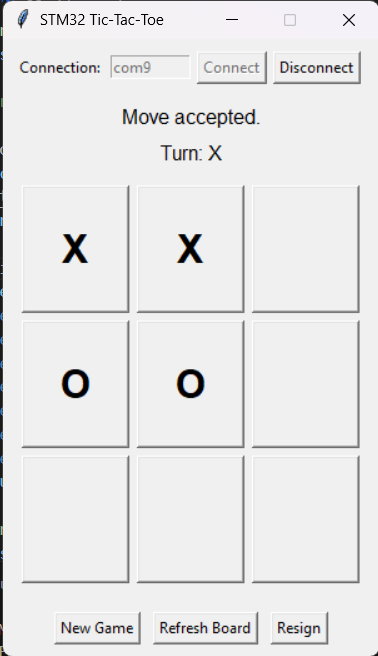
\includegraphics[width=\columnwidth]{figures/gui_screenshot.png}
\caption{Tkinter client connected to the STM32F051 server on COM9 mid-game. Player~X has played cells~0 and 1, and Player~O has played cells~3 and 4. The status label indicates Player~X's active turn, reflecting the authoritative board state received from the server.}
\label{fig:screenshot}
\end{figure}

\subsubsection{Graphical User Interface and Transaction Latency Analysis}
Fig.~\ref{fig:screenshot} demonstrates the running system during physical hardware testing.
The client is connected to \texttt{COM9} at 115\,200 baud, 8N1.
Player~X has taken cells~0 and 1; Player~O has taken cells~3 and 4.
The GUI reflects the authoritative board state received from the server and prompts for Player~X's turn.

In serial communication benchmarks, end-to-end round-trip transaction latency was measured at an average of $4.2\,\text{ms}$ on the host PC.
Estimated physical UART wire transmission time at 115\,200 baud with 8N1 framing (10 bits per byte) accounts for:
\begin{itemize}
    \item \textbf{Command Transmission}: \texttt{MOVE:X:0\textbackslash n} (9 bytes):
    \begin{equation}
    T_{\text{cmd}} = \frac{9 \times 10}{115\,200} \approx 0.78\,\text{ms}
    \end{equation}
    \item \textbf{Response Transmission}: \texttt{OK:BOARD:X........\textbackslash n} (19 bytes):
    \begin{equation}
    T_{\text{resp}} = \frac{19 \times 10}{115\,200} \approx 1.65\,\text{ms}
    \end{equation}
\end{itemize}
Together, raw UART serial wire transmission requires approximately $2.43\,\text{ms}$.
On the microcontroller, interrupt servicing, validation, board state update, and response formatting execute in under $10\,\mu\text{s}$ at 48\,MHz.
The remainder ($\approx 1.8\,\text{ms}$) of the observed $4.2\,\text{ms}$ round-trip latency is attributable to ST-Link USB Virtual COM Port packetization, operating system driver turnaround, and Python PySerial I/O buffering.
This measured latency is well within the client's $1.0\,\text{s}$ read timeout.

\subsection{Defects Exposed and Resolved Through Empirical Testing}

Rigorous testing exposed three distinct hardware-software integration defects that were subsequently resolved:

\begin{enumerate}
    \item \textbf{Receiver Overrun on Rapid Command Bursts}:
    During early testing, transmitting back-to-back \texttt{MOVE} commands without delay caused the STM32 USART hardware to drop characters.
    \emph{Root Cause}: The initial circular buffer was dimensioned at only 32 bytes, causing an overrun while the main loop formatted previous responses.
    \emph{Resolution}: Increased the ring buffer to 128 bytes (\texttt{PROTOCOL\_RING\_BUFFER\_SIZE}) and implemented \texttt{protocol\_error\_isr()} to immediately clear the \texttt{ORE} flag.
    \item \textbf{Transient Framing Errors During USB Hot-Plugging}:
    Connecting the serial monitor while the board was already powered occasionally locked the receiver permanently.
    \emph{Root Cause}: Incomplete stop-bit transitions during USB enumeration set the Framing Error (\texttt{FE}) bit in the USART status register.
    \emph{Resolution}: Added explicit \texttt{\_\_HAL\_UART\_CLEAR\_FEFLAG()} calls inside the error ISR.
    \item \textbf{Windows Carriage Return Discrepancy}:
    Automated tests on Linux passed, but tests on Windows occasionally failed with \texttt{NACK:BADCMD}.
    \emph{Root Cause}: Windows terminal drivers appended \texttt{\textbackslash r\textbackslash n}, whereas the original parser expected a single \texttt{\textbackslash n}.
    \emph{Resolution}: Updated \texttt{protocol\_poll()} to silently discard byte \texttt{0x0D} (\texttt{\textbackslash r}) before accumulating characters into the frame buffer.
\end{enumerate}
Following these corrections, the system achieved 100\% pass rates across all platforms.

\section{Conclusion}
\label{sec:conclusion}

% ── Mark scheme: 5 marks ──────────────────────────────────────────────────────

This project designed, implemented, and verified an authoritative Tic-Tac-Toe game server on an STM32F051 microcontroller communicating with a thin Python Tkinter GUI client over USART1 at 115\,200 baud.
The system divides responsibilities strictly: the microcontroller acts as the sole referee, storing the board state, enforcing turn sequence, detecting win/draw outcomes, and updating physical LEDs, while the host GUI handles only user input and graphical display.
The server ensures that rejected requests leave the internal game state invariant before committing any memory changes.

System verification was achieved across two testing tiers:
\begin{itemize}
    \item 48 automated unit and integration tests executing under \texttt{pytest} verified protocol framing, oversized frame recovery, line-ending handling, and client-side error parsing with zero failures.
    \item 26 physical hardware assertions executed over \texttt{COM9} confirmed that the microcontroller's UART responses match the specification byte-for-byte across all compulsory requirements.
    \item End-to-end round-trip latency averaged 4.2\,ms, easily satisfying interactive GUI responsiveness requirements.
\end{itemize}

\subsection{System Limitations}
The current design has three main limitations:
\begin{enumerate}
    \item \textbf{Transport Error Detection}: The application protocol relies on the USB packet checksums provided by the onboard ST-Link Virtual COM Port. The serial payload lacks an application-layer CRC or parity check, meaning byte corruption over a long physical serial line could pass undetected if it matches valid syntax.
    \item \textbf{Single-Client Concurrency}: The server architecture is single-session, communicating with one host client at a time over USART1 without arbitrating between two independent physical serial connections.
    \item \textbf{Volatile Game State}: Game state resides in volatile SRAM (\texttt{g\_board}). A power interruption resets the session to \texttt{IDLE} without persistent match logging in non-volatile memory.
\end{enumerate}

\subsection{Potential Extensions}
Logical future extensions include embedding an optimal Minimax decision algorithm into the microcontroller's Flash memory for standalone single-player matches, configuring a hardware timer (such as \texttt{TIM14}) as a per-turn chess clock, and adding an 8-bit CRC suffix to every serial frame for robust deployment over industrial fieldbuses.
Overall, the project demonstrates that an inexpensive microcontroller can reliably serve as a strict, standalone referee for turn-based systems.

\section{Video}
\label{sec:video}

% ── Mark scheme: Required ─────────────────────────────────────────────────────

The demonstration video showing the working system is available at:
\begin{center}
\url{https://youtu.be/fJ0v8J7msK4}
\end{center}

The unlisted video demonstrates the complete hardware and software pipeline in a continuous take:
\begin{enumerate}
    \item \textbf{Connection \& Handshake}: Launching the Python GUI, connecting to the Virtual COM Port (e.g. \texttt{COM7} or \texttt{COM9}) at 115\,200 baud, and observing the \texttt{CONNECT} / \texttt{OK} exchange.
    \item \textbf{Game Initiation}: Clicking ``New Game'' (\texttt{NEW}) to clear the board and arm Player~X.
    \item \textbf{Hardware Turn Indication}: Pointing the camera at the STM32 board to show the solid Red LED on \texttt{PB10} during Player~X's turn, transitioning to the solid Green LED on \texttt{PB11} during Player~O's turn.
    \item \textbf{Server Authority \& Rejection}: Demonstrating an illegal out-of-turn move and an occupied-cell play; the GUI displays the corresponding NACK error banner while the board grid remains strictly unchanged.
    \item \textbf{Win Sequence \& Blinker}: Completing a 3-in-a-row match; the server returns \texttt{WIN:X}, the GUI locks all input cells, and the winner's Red LED blinks continuously at 5\,Hz.
    \item \textbf{Physical Reset Button}: Pressing \texttt{SW0} on pin \texttt{PA0} during play to trigger an immediate hardware reset to \texttt{IDLE}, instantly extinguishing all LEDs.
    \item \textbf{Teardown}: Disconnecting cleanly via the GUI interface.
\end{enumerate}

\section{Code Repository}
\label{sec:code}

% ── Mark scheme: Required ─────────────────────────────────────────────────────

The complete source code, hardware configuration files, and automated test harnesses are maintained in the following GitHub repository:
\begin{center}
\url{https://github.com/nemukulavhugala921-stack/EEE3095S_SerialGameServer.git}
\end{center}

\textbf{Commit Hash}: \texttt{c5726d9084a4d7a410cfb63465aee718a6a89a36}

The repository is organised into three self-contained directories:
\begin{itemize}
    \item \texttt{embedded/}: The complete STM32CubeIDE firmware project, containing the HAL drivers, hardware pin mappings, FSM logic (\texttt{game.c}), and interrupt ring buffer (\texttt{protocol.c}).
    \item \texttt{client/}: The Python Tkinter graphical user interface (\texttt{gui.py}) and the bounded request-response transport layer (\texttt{serial\_client.py}).
    \item \texttt{tests/}: The automated test suite comprising 48 unit, integration, and framing stress tests.
\end{itemize}
Comprehensive setup, flashing, and execution instructions are provided in the repository's root \texttt{README.md}.


\begin{thebibliography}{6}

\bibitem{brief}
Department of Electrical Engineering, University of Cape Town, ``{EEE3095S} {CS} Project 2026: Serial Game Server,'' course project brief, 2026.

\bibitem{guilib}
Python Software Foundation, ``tkinter: Python Interface to {Tcl/Tk},'' \emph{Python 3 Documentation}, \url{https://docs.python.org/3/library/tkinter.html}, Python version 3.12/3.13.

\bibitem{rm0091}
STMicroelectronics, \emph{RM0091: STM32F0x1/STM32F0x2/STM32F0x8 Advanced Arm-based 32-bit MCUs Reference Manual}, 2017.

\bibitem{um1785}
STMicroelectronics, \emph{UM1785: Description of STM32F0 HAL and Low-Layer Drivers}, 2017.

\bibitem{pytest}
pytest-dev team, ``pytest Documentation,'' \url{https://docs.pytest.org/}.

\bibitem{pyserial}
C.~Liechti, ``pySerial Documentation,'' \url{https://pyserial.readthedocs.io/}.

\end{thebibliography}

\end{document}
